Model based design has been quite successful in the industry. 
Tools like \SIMULINK are often used to create models describing hybrid
dynamical systems. Testing such systems for safety properties remains
a hard problem, and the current approaches consist of either guided
testing using numerical simulations or translating to hybrid automata.
We now suggest an approach which lies in the middle.

In this work we propose a two step process for searching violations of
the properties. This involves (a) learning a piece-wise affine model
and (b) exhaustively searching it for violations. It must be noted
that the violation found in the model might not be valid in the
original system, depending on the accuracy of the model.
% concretizing the violation in the original system.

The piece-wise affine model is the aggregation of affine maps, each
approximating observed local behavior of the system.  The model is
discrete time and `relational'. It relates the states reachable in a
fixed time step $\Delta$ to a given state.

In our previous work~\cite{zutshi2014multiple}, we analyzed systems by
restricting ourselves to their black box semantics. This enabled us to
reason about the state-space reachability of the system without a
direct analysis of its structure. Using a coarse abstraction which we
searched on-the-fly, we could observe the local dynamics as required.
This gave us an efficient procedure to find abstract counter-examples.
However, to concretize the counter-examples, a `closer look' or
refinement of the abstraction is required. The grid based state-space
abstraction was refined by splitting the relevant cells (abstract
states) into smaller ones. As noted previously, due to the curse of
dimensionality, such a uniform splitting is an expensive operation,
and can not scale to higher dimensions.

We further our exploration of trajectory segment based methods; and
explore an alternative approach to overcome the explosion in abstract
states. Instead of selectively refining the abstraction, we compute a
model of the black box system and use bounded model checking to find a
concrete counter-example in the model. Due to modeling errors, this
might not be reproducible in the original black-box system. We then
use this counter-example to guide the search towards a counter-example
in the original system.

More specifically, we use regression to quantitatively estimate the
discovered relations, which were witnessed by trajectory segments, by
affine maps. These maps approximate locally observed behaviors, which
are incorporated into the sampled reachability graph as edge
annotations.  The resulting graph or the Piece-Wise Affine (PWA)
relational model can be interpreted as an infinite state discrete
transition system and model checked for time bounded safety
properties. A counter-example if found, can indicate the presence of a
violation in the system.
%Furthermore, using linear programming, we can over-approximate the
%neighbhourhood of the counter-example in the model.

% Towards the end of the chapter, we discuss extensions to data driven
% approaches (instead of simulator driven), where instead of a
% simulator, a fixed set of data is provided as the behavioral
% description of the system. Using a combination of relational modeling,
% and program analysis we outline the future work for falsifying
% properties of SDCS.


\section{Relational Modeling}

We now describe how relational models can be computed for a given
black box system by enriching the abstract reachability graph obtained
by scatter-and-simulate. We first formalize the notion of an enriched
graph, and then show how they can be interpreted as a PWA transition
system using $k$-relational modeling.

\subsection{Abstract Enriched Graph}

The existential abstraction relation in \chapref{abs} was defined as
follows:
\[
%\exists \x\in\C. \exists \x'\in\C'. \x'=\simulate(\x, \tau) \iff \C\rel{\tau}\C'
    C \areach{t} C' \iff \exists \x \in C.\ \exists \x' \in C'.\ \x \areach{t} \x'
\]
The abstract relation $\areach{t}$ can be enriched by incorporating
the affine relation between $\x$ and $\x'$. For an arbitrary dynamical
system, such a relation can be rarely represented using an exact affine map.
This is due to the presence of non-linear and hybrid behaviors. But,
an affine map can always be estimated with an error.

If the system dynamics are completely specified in the form of a white
box model, we can use first order approximations to find the affine
expressions for the relations. Using a tool like \flowstar, we can
obtain sound over-approximate affine maps of the form $A\x + [\vb^l,
\vb^h]$, where $[\vb^l,\vb^h]$ denotes the interval of vectors, such
that, every element $b_i$ of the vector $\vb$ is contained in the
respective scalar interval $b_i\in[b^l_i,b^h_i]$.

For the case of black box systems, such a sound approximation is not
possible. Instead, we rely on a statistical method like simple linear
regression to estimate the affine map $\amap: A\x + \vb$. We then
estimate the error $\delta$ and generalize $\amap$ to an interval
affine map as before $\amap: A\x + \vb + \delta$.  Finally, we get an
abstraction with the below relation
\[
    C \areach{f} C' \iff \exists \x \in C.\ \exists \x' \in C'.\ \x' \in A\x + \vb \pm \delta.
    %C \areach{A\x+\vb+\delta} C' \iff \exists \x \in C.\ \exists \x' \in C'.\
\]

However, in the presence of complex non-linear behavior, using a
single affine map can lead to a poor approximation. To increase the
precision, one can use more than one affine map. Let us denote this set as
$R_{(C,C')}$ (ref.~\secref{ovw}).
\[
    R_{(C,C')}(\x,\x'): \setof{f_i \;|\; \exists \x \in C.\ \exists \x' \in C'.\ \x' \in f_i(\x)}
\]

\begin{figure}[!htbp]
\begin{center}
\tikzstyle{line} = [thick]
\tikzstyle{arw} = [->, thick,>=stealth,shorten <=2pt, shorten >=2pt]
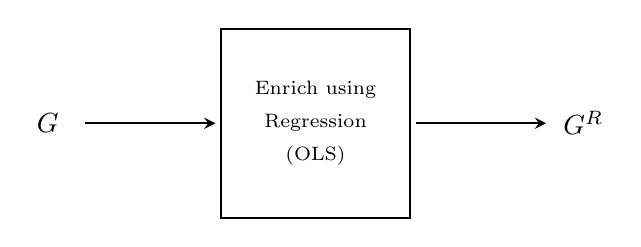
\begin{tikzpicture}

    \draw [line] (-1.2,-1.2) rectangle (1.2,1.2);
    \draw[arw] (-3,0) -- (-1.2,0);
    \draw[arw] (1.2,0) -- (3,0);

\node at (-3.4,0) {$G$};
\node at (3.4,0) {$G^R$};
\node[align=center] at (0, 0) {\scriptsize Enrich using \\ \scriptsize Regression \\ \scriptsize(OLS)};

\end{tikzpicture}
\end{center}
\vspace*{-.3cm}
\caption{Using OLS, $G^R$ is computed by determining the appropriate
$R_{(C,C')}$ for each edge of $G$.}
\label{fig:enrichment}
\vspace*{-.3cm}
\end{figure}

As shown in \figref{enrichment}, we use OLS to compute an enrichment
of the abstraction graph $G$. For every edge $(C,C') \in edges(G)$,
the set of relations $R_{(C,C')}(\x,\x')$ is computed. The semantics
of the enriched edge are clearly non-deterministic. Form a state $\x
\in C$, any $f_i\in R_{(C,C')}$ can be taken as long as $\x' \in C$'
is satisfied. This interpretation results in an infinite state
transition system. We now detail the construction of the set
$R_{(C,C')}$ using $k$-relational modeling.

% We now compute a PWA model for a given black box system by estimating
% the dynamics using OLS. We can estimate the affine relations between
% every cell, but as discussed in ~\chapref{abs}, it is a futile
% approach.  Instead, we use the same heuristic as before:
% scatter-and-simulate, to select the cell relations for estimation. We
% build the reachability graph as before, but in addition, annotate each
% edge with the values of estimated $A$, $\vb$, and $\delta$ for the
% respective relation. The reachability graph thus computed, is a
% transition system. Using off-the-shelf bounded model checkers, we
% reason about the system's safety properties.


\subsection{$k$ - Relational Modeling}

\begin{figure}[!htbp]
\vspace*{-.2cm}
\begin{center}
\tikzstyle{line} = [thick]
\tikzstyle{arw} = [->, thick,>=stealth,shorten <=2pt, shorten >=2pt]
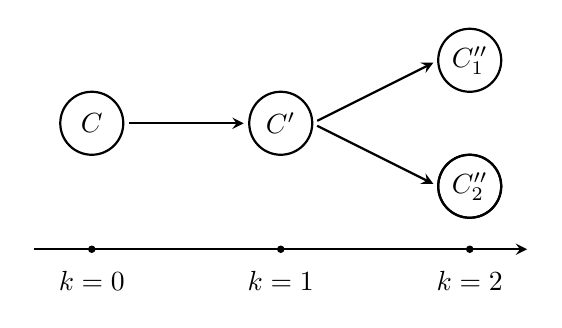
\begin{tikzpicture}

\begin{scope}[scale=0.8]
\draw [line] (-1.0,0) circle (0.5);
\draw [line] (-4.0,0) circle (0.5);
\draw [line] (2.0,1) circle (0.5);
\draw [line] (2.0,-1) circle (0.5);
\draw[arw] (-0.5,0) -- (1.5,1.0);
\draw[arw] (-0.5,0) -- (1.5,-1.0);
\draw[arw] (-3.5,0) -- (-1.5,0.0);
\node at (-4.0,0) {$C$};
\node at (-1.0,0) {$C'$};
\node at (2.0,1.0) {$C''_1$};
\node at (2.0,-1.0) {$C''_2$};
\draw [line] (2.0,-1) circle (0.5);
\draw[arw] (-5.0,-2.0) -- (3.0,-2.0);
\node at (-4.0,-2.5) {$k=0$};
\node at (-1.0,-2.5) {$k=1$};
\node at (+2.0,-2.5) {$k=2$};
\draw [fill=black] (-4.0,-2.0) circle (0.05);
\draw [fill=black] (-1.0,-2.0) circle (0.05);
\draw [fill=black] (2.0,-2.0) circle (0.05);

\end{scope}
\end{tikzpicture}
\end{center}
\vspace*{-.3cm}
\caption{Nodes/Cells of $G$ shown along with increasing values of $k$.}
\label{fig:k-rel}
\vspace*{-.3cm}
\end{figure}

Given a $G$, when computing the set of relations for an edge $R$, we
consider only the set of abstract states reachable at a specific time
step.  Intuitively, one might consider the states reachable in one
time step $\Delta$.  However, such a process can be generalized by
looking at the states reachable at ${0\Delta, 1\Delta, \ldots,
k\Delta}$ time steps.

Using \figref{k-rel}, we illustrate this notion. To compute
$R_{(C,C')}$, we
split the data set $D(C,C')$ consisting of trajectory segments (of time lengths
$k\Delta$) as follows.  We observe the local behavior of the system by
noting the evolution of the system $\System$ from a state $\x(t)
\in C$ for a time length dependant on $k$. For
\begin{itemize}
    \item{$k=0$}: we observe all trajectory segments of length $\Delta$.
    \item{$k=1$}: we observe trajectory segments of length $\Delta$, which satisfy $\x(t+\Delta) \in C'$.
    \item{$k=2$}: we observe trajectory segments of length $2\Delta$,
        and split them in two sets (a) and (b) on the basis of the
        cells reached at time $(t+\Delta)$ and $(t+2\Delta)$.
        \begin{enumerate}[(a)]
            \item $\x(t+\Delta) \in C' \land \x(t+2\Delta) \in C''_1$
            \item $\x(t+\Delta) \in C' \land \x(t+2\Delta) \in C''_2$
        \end{enumerate}
    \item{$k=n$}: we observe trajectory segments of length $n\Delta$,
        and split them in to multiple sets on the basis of the cells
        reached at time $(t+\Delta),\; (t+2\Delta),\;
        \ldots,\;(t+n\Delta)$.
\end{itemize}

$k$-relational modeling can be understood as a heuristic, which uses
the underlying abstraction to differentiate behaviors of the system
which `diverge' (or are revealed to be `distinct' at a future time).
Such a heuristic can be useful in increasing the precision of the
learnt affine maps.  We now formalize this notion for $k=0$, $1$, and
$n$ and illustrate using examples.

\mypara{$0$-Relational Model}

\begin{figure}[!htbp]
\begin{center}
\tikzstyle{line} = [thick]
\tikzstyle{arw} = [->, thick,>=stealth,shorten <=2pt, shorten >=2pt]
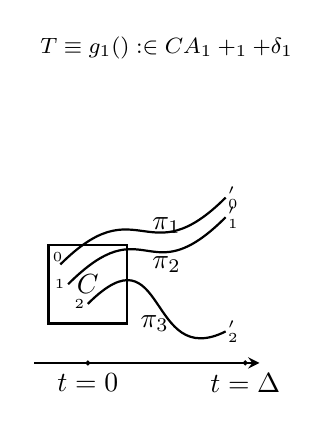
\begin{tikzpicture}
\begin{scope}[scale=0.5]

    \draw [line] (-1.0,-1.0) rectangle (1.0,1.0);
    %\draw [line] (3.0,1.0) rectangle (5.0,3.0);
    %\draw [line] (3.0,-3.0) rectangle (5.0,-1.0);
    \draw [line] (-0.7,0.5) .. controls +(2.0,2.0) and +(-2.0,-2.0) ..  (3.5,2.2);
    \draw [line] (-0.5,0.0) .. controls +(2.0,2.0) and +(-2.0,-2.0) ..  (3.5,1.7);
    \draw [line] (-0.0,-0.5) .. controls +(2.0,2.0) and +(-2.0,-1.0) ..  (3.5,-1.2);

\node at (0.0, 0.0) {$C$};
\node at (-0.75,0.7) {\scriptsize{$\x_0$}};
\node at (3.7,2.2) {\scriptsize{$\x_0'$}};
\node at (-0.7,0.0) {\scriptsize{$\x_1$}};
\node at (3.7,1.7) {\scriptsize{$\x_1'$}};
\node at (-0.2,-0.5) {\scriptsize{$\x_2$}};
\node at (3.7,-1.2) {\scriptsize{$\x_2'$}};
\node at (2,1.5) {$\pi_1$};
\node at (2,0.5) {$\pi_2$};
\node at (1.7,-1) {$\pi_3$};
\draw[arw] (-1.5,-2.0) -- (4.5,-2.0);
\node at (0,-2.5) {$t=0$};
\node at (4,-2.5) {$t=\Delta$};
\draw [fill=black] (0.0,-2.0) circle (0.05);
\draw [fill=black] (4.0,-2.0) circle (0.05);

\end{scope}
\begin{scope}[xshift=0,yshift=3.0cm,scale=0.5]
    \node at (2,0) {\footnotesize $\scr{T} \equiv g_1(\x):\vx \in C
    \implies A_1\vx + \vb_1 + \delta_1$};
\end{scope}

\end{tikzpicture}
\end{center}
\vspace*{-.3cm}
\caption{All the trajectory segments will be used to construct the
model; $\ds = \setof{\pi_1, \pi_2, \pi_3}$.}
\label{fig:k0}
\vspace*{-.3cm}
\end{figure}

When $k=0$, the $0$-relational model is a PWA transition system which only
defines the evolution of states $\x$, and does not specify the
reachable cell. The guard predicates of the relations are defined over
cells: $g_i(\x): \x \in C_i$ while $g'_i(\x'): True$.

We use regression to estimate the dynamics for the outgoing trajectory
segments form a cell $C$. Hence, the data set $\ds$ for the regression
includes all trajectory segments beginning from the same cell
\[
    \ds = \setof{\pi_t | start(\pi_t) \in C}.
\]
This includes trajectory segments ending in different cells, as shown
in ~\figref{k0}. For $N$ cells, this results in a $\rho$ with $N$ transition relations.
\begin{equation*}
    \scr{T} = \left\{
        \begin{array}{ll}
            g_1(\x):\vx \in C_1 \implies A_1\vx + \vb_1 + \delta_1\\
            \ldots \\
            g_n(\x):\vx \in C_n \implies A_n\vx + \vb_n + \delta_n\\
        \end{array}
    \right.
\end{equation*}

Note that this can be quite imprecise when the cells are big,
containing regions of state-space with complex dynamics. This is true
for both non-linear systems and hybrid dynamical system, where a cell
can contain two or more modes with differing continuous dynamics.

\mypara{$1$-Relational Model}

\begin{figure}[!htbp]
\begin{center}
\tikzstyle{line} = [thick]
\tikzstyle{arw} = [->, thick,>=stealth,shorten <=2pt, shorten >=2pt]
\begin{tikzpicture}
\begin{scope}[scale=0.5]

    \draw [line] (-1.0,-1.0) rectangle (1.0,1.0);
    \draw [line] (3.0,1.0) rectangle (5.0,3.0);
    \draw [line] (3.0,-3.0) rectangle (5.0,-1.0);
    \draw [line] (-0.7,0.5) .. controls +(2.0,2.0) and +(-2.0,-2.0) ..  (3.5,2.2);
    \draw [line] (-0.5,0.0) .. controls +(2.0,2.0) and +(-2.0,-2.0) ..  (3.5,1.7);
    \draw [line] (-0.0,-0.5) .. controls +(2.0,2.0) and +(-2.0,-1.0) ..  (3.5,-1.2);

\node at (0.0, 0.0) {$C$};
\node at (4.0, 2.0) {$C'_1$};
\node at (4.0, -2.0) {$C'_2$};
\node at (-0.75,0.7) {\scriptsize{$\x_0$}};
\node at (-0.7,0.0) {\scriptsize{$\x_1$}};
\node at (-0.2,-0.5) {\scriptsize{$\x_2$}};
\node at (3.3,2.5) {\scriptsize{$\x_0'$}};
\node at (3.7,1.5) {\scriptsize{$\x_1'$}};
\node at (3.7,-1.5) {\scriptsize{$\x_2'$}};
\node at (2,1.5) {$\pi_1$};
\node at (2,0.5) {$\pi_2$};
\node at (1.7,-1) {$\pi_3$};
\draw[arw] (-1.5,-3.5) -- (5.5,-3.5);
\node at (0,-4.0) {$t=0$};
\node at (4,-4.0) {$t=\Delta$};
\draw [fill=black] (0.0,-3.5) circle (0.05);
\draw [fill=black] (4.0,-3.5) circle (0.05);

\end{scope}
\begin{scope}[xshift=0,yshift=4.0cm,scale=0.5]
    \node at (2,0) {\begin{minipage}{\linewidth}
    \footnotesize \begin{equation*}
        \scr{T} = \left\{
        \begin{array}{ll}
            g_1(\x):\vx \in C \land g'_1(\x):\vx \in C'_1 \implies A_1\vx + \vb_1 + \delta_1\\
            g_2(\x):\vx \in C \land g'_2(\x):\vx \in C'_2 \implies A_2\vx + \vb_2 + \delta_2
        \end{array}
    \right.
\end{equation*}
\end{minipage}};
\end{scope}

\end{tikzpicture}
\end{center}
\vspace*{-.3cm}
\caption{The data gets split into two sets $\ds_1 = \setof{\pi_1,
    \pi_2}$ and $\ds_2 = \setof{\pi_3}$ and two relations:
    $R_{(C,C'_1)}$ and $R_{(C,C'_2)}$, each with one affine map, are constructed.}
%Cardinality($R_{(C,C')}$) = $2$.}
\label{fig:k1}
\vspace*{-.3cm}
\end{figure}


% \begin{scope}[xshift=0,yshift=4.0cm,scale=1]
%     \node at (2,0) {\footnotesize $\begin{equation*}
%     \scr{T} = \left\{
%         \begin{array}{ll}
%             g_1(\x):\vx \in C \land g'_1(\x):\vx \in C'_1 \implies A_1\vx + \vb_1 + \delta_1\\
%             g_2(\x):\vx \in C \land g'_2(\x):\vx \in C'_2 \implies A_2\vx + \vb_2 + \delta_2
%         \end{array}
%     \right.
% \end{equation*}$};
% \end{scope}

To improve the preciseness of learnt dynamics, we include the
reachability relation in the
regression. For every relation $C\areach{t}C'$, the data set $\ds$ is
comprised only of trajectory segments $\pi_t$ which start and end in
the same set of cells.
\[
    \ds = \setof{\pi_t | start(\pi_t) \in C \land end(\pi_t) \in C'}.
\]
For $N$ edges in $G$, $1$-relationalization results in a $\rho$ with
$N$ transition relations.

\figref{k1} illustrates the $k=1$ refinement of the case shown in
\figref{k0}. The data set $\ds$ is split into two data sets $\ds_1
= \setof{\pi_1, \pi_2}$ and $\ds_2 = \setof{\pi_3}$, using which, two
relations are constructed. The resulting $1$-relational model
is at least as precise as the corresponding $0$-relational model.

\mypara{$k$-Relational Model}

\begin{figure}[!htbp]
\begin{center}
\tikzstyle{line} = [thick]
\tikzstyle{arw} = [->, thick,>=stealth,shorten <=2pt, shorten >=2pt]
\begin{tikzpicture}
\begin{scope}[scale=0.5]

    \draw [line] (-1.0,-1.0) rectangle (1.0,1.0);
    \draw [line] (3.0,1.0) rectangle (5.0,3.0);
    %\draw [line] (3.0,-3.0) rectangle (5.0,-1.0);
    \draw [line] (7.0,1.0) rectangle (9.0,3.0);
    \draw [line] (7.0,-3.0) rectangle (9.0,-1.0);
    \draw [line] (-0.7,0.5) .. controls +(2.0,2.0) and +(-2.0,-2.0) .. (3.5,2.2) .. controls +(2.0,2.0) and +(-2.0,-2.0) .. (8.5,1.8) ;
    \draw [line] (-0.5,0.0) .. controls +(2.0,2.0) and +(-2.0,-2.0) .. (3.5,1.7) .. controls +(2.0,2.0) and +(-2.0,-2.0) .. (8.5,-2.2) ;

%     \draw [line] (-0.7,0.5) .. controls +(2.0,2.0) and +(-2.0,-2.0) ..  (3.5,2.2);
%     \draw [line] (-0.5,0.0) .. controls +(2.0,2.0) and +(-2.0,-2.0) ..  (3.5,1.7);

    %\draw [line] (-0.0,-0.5) .. controls +(2.0,2.0) and +(-2.0,-1.0) ..  (3.5,-1.2);

\node at (0.0, 0.0) {$C$};
\node at (4.0, 2.0) {$C'_1$};
\node at (8.0, 2.0) {$C''_1$};
\node at (8.0, -2.0) {$C''_2$};
%\node at (4.0, -2.0) {$C'_2$};
\node at (-0.75,0.7) {\scriptsize{$\x_0$}};
\node at (-0.7,0.0) {\scriptsize{$\x_1$}};
%\node at (-0.2,-0.5) {\scriptsize{$\x_2$}};
\node at (3.3,2.5) {\scriptsize{$\x_0'$}};
\node at (3.7,1.5) {\scriptsize{$\x_1'$}};
%\node at (3.7,-1.5) {\scriptsize{$\x_2'$}};
\node at (8.7,1.6) {\scriptsize{$\x_0''$}};
\node at (8.5,-2.7) {\scriptsize{$\x_1''$}};
\node at (2,1.5) {$\pi_1$};
\node at (2,0.5) {$\pi_2$};
\draw[arw] (-1.5,-3.5) -- (9.5,-3.5);
\node at (0,-4.0) {$t=0$};
\node at (4,-4.0) {$t=\Delta$};
\node at (8,-4.0) {$t=2\Delta$};
\draw [fill=black] (0.0,-3.5) circle (0.05);
\draw [fill=black] (4.0,-3.5) circle (0.05);
\draw [fill=black] (8.0,-3.5) circle (0.05);
\end{scope}

\begin{scope}[xshift=0,yshift=4.0cm,scale=0.5]
    \node at (4,0) {\begin{minipage}{\linewidth}
        \footnotesize \begin{equation*}
    \scr{T} = \left\{
        \begin{array}{ll}
            g_1(\x):\vx \in C \land g'_1(\x):\vx \in C'_1 \implies A_1\vx + \vb_1 + \delta_1\\
            g_1(\x):\vx \in C \land g'_1(\x):\vx \in C'_1 \implies A_2\vx + \vb_2 + \delta_2
        \end{array}
    \right.
\end{equation*}
\end{minipage}};
\end{scope}

\end{tikzpicture}
\end{center}
\vspace*{-.3cm}
\caption{The $k=2$ refinement further splits the data set $\ds_1$
    into two sets $\ds_{11} = \setof{\pi_1}$ and $\ds_{12} =
    \setof{\pi_2}$ and $R_{(C,C'_1)}$ now has two affine maps,
    non-deterministically defining the system behavior.}
\label{fig:k2}
\vspace*{-.3cm}
\end{figure}

Finally, we generalize the relational models to $k$-relational PWA
models. A $k$-relational model is constructed by using $k$ length
\textit{connected} segmented trajectories. A segmented trajectory $\SegTraj$ is
\textit{connected} iff its cost $\cost(\SegTraj) = 0$.

Two $\SegTraj:\tupleof{\pi_{t_1}, \ldots, \pi_{t_k}}$ and
$\SegTraj':\tupleof{\pi'_{t_1}, \ldots, \pi'_{t_k}}$ are
\textit{similar} if their trajectory segments have the same sequence
of cell traversals $\tupleof{C_1, C_2, \ldots, C_k}$, \ie
\[
    \forall i\in\setof{1 \ldots k}.
    start(\pi_{t_i}) \in C_i
    \land start(\pi'_{t_i}) \in C_i
    \land end(\pi_{t_i}) \in C_{i+1}
    \land end(\pi'_{t_i}) \in C_{i+1}
\]

For every cell $C$ in the reachability graph, we construct a data set
$\ds$ by collecting $\pi_{t_i}$, such that they are the first segment of $k$
length \textit{connected} and \textit{similar} segmented trajectories.
%\[
%    \ds = \setof{\pi_{\tau_i} |
%        \pi_{\tau_i}
%        start(\pi_{\tau_{i}}) \in C_i
%        \land
%        end(\pi_{\tau_{i}}) \in C_i}
%\]

\figref{k2} illustrates the $k=2$ refinement on \figref{k1}.

\section{Bounded Model Checking Black Box Systems}
% include an algorithm
We now describe the entire procedure in three steps.
\begin{enumerate}
    \item Given a black box system $\System$ specified by
        $\simulate_\System$, we
        use scatter-and-simulate with ($\Delta$-length) trajectory
        segments to sample a finite reachability graph
        $\scr{H}(\Delta)$.
    \item Using regression, we enrich the graph relations and annotate
        the edges with the estimated affine maps.
    \item Interpreting the directed reachability graph as a transition
        system, we use a bounded model checker to find fixed length
        violations to safety properties.
\end{enumerate}


\section{An Example: Van der Pol Oscillator}

We now describe the above using the Van der Pol oscillator benchmark
presented in \secref{math-dyn-sys}. Simulations generated using
uniformly random samples are shown in \figref{vdp-cont}. We want to
check the property $P_3$, indicated by the red box, given the initial
set indicated by the green box. The abstraction is defined by
$\quant_{0.2}(\x)$, which results in an evenly gridded state-space,
where each cell is of size $0.2 \times 0.2$ units.
Scatter-and-simulate is then used to construct the abstract graph $G$,
using $2$ samples per cell and the time step $\Delta = 0.1s$. The
complete process follows.

\begin{enumerate}
    \item{\emph{Abstract}} Consider an implicit abstraction induced by the quantization
    function $\quant_\epsilon(\x)$. The corresponding reachability
    graph $\scr{H}(\Delta)$ (with time step $\Delta$) is given by
    $\tupleof{\scr{C},\areach{\Delta}, \scr{C}_0, \scr{C}_u}$.
\item{\emph{Discover}}: Using scatter-and-simulate, enumerate a finite number
    of cells (vertices) and the relations (edges) of the graph
    $\scr{H}(\Delta)$. Associate the set of generated trajectory
    segments with their respective originating cells using a map $D:C
    \mapsto \setof{\pi | start(\pi) \in C}$. The discovered
    abstraction is show in \figref{vdp-abs}. As mentioned, red cells
    are unsafe and green cells are initial cells.
\item{\emph{Relationalize}} For each cell $C$, perform regression analysis on
    the respective set of trajectory segments $D(C)$, and compute a
    set of affine relations $R_{C,C'}(\x,\x')$ between $\x \in C$ and $\x'
    \in C'$ s.t., $\text{edge} (C,C') \in \scr{H}(\Delta)$. Annotate
    each edge in the graph $\scr{H}(\Delta)$ with the respective
    relation.

    \figref{vdp-map} shows the cells and the trajectory segments which
    are part of the data sets constructed using the $1$-relational
    modeling. Against each cell, its unique identifier (integer
    co-ordinate) is mentioned.  Finally, \figref{vdp-graph} and
    \tabref{vdp-pwa} show the enriched graph $G^R$ with its transition
    relations. Note that self loops result when an observed trajectory
    segment has its $start$ and $end$ states in the same cell.

\item{\emph{Model Check}} The graph $\scr{H}(\Delta)$ can now be viewed as a
    transition system $\tupleof{C,\x,\scrT,C_0,\HybridStates_0}$,
    where $C \in vertices(\scr{H}(\Delta))$ and $\x \in
    \HybridStates$. A transition $\tau \in \scrT$ is of the form
    $\tupleof{C, C',\rho_{\tau}}$, where $\rho_{\tau}(\x,\x')
    \subseteq \setof{R_{(C,C')}(\x,\x') |( C,C') \in
    edge(\scr{H}(\Delta))}$.
\item{\emph{Check Counter-example}} The infinite state (but finite location) transition system can
    be model checked to find a concrete counter-example, which if
    exists, can indicate the existence of a similar trace in the
    original black-box system $\System$. The latter check is carried
    out as before, using the numerical simulation function
    $\simulate$. For the given example, the model checker is unable to
    find a counter-example.
\end{enumerate}

\inclfig[width=0.75\linewidth]{vdp_cont_traces.png}{Van der
Pol: continuous trajectories. Red and green boxes indicate unsafe and
initial sets.}
\label{fig:vdp-cont}

\inclfig[width=0.75\linewidth]{vdp_abs.png}{The discovered
abstraction $\scr{H}(0.1)$. Red cells are unsafe cells and green cells are
initial cells.}
\label{fig:vdp-abs}

\inclfig[width=\linewidth]{vdp_disc_map.png}{Cells and
trajectory segments used by $1$-relational modeling.}
\label{fig:vdp-map}

\inclfig[width=0.40\linewidth]{vdp_graph.png}{Enriched
graph $G^R$. The affine maps $f$ for the transition relations are show
in \tabref{vdp-pwa}.}
\label{fig:vdp-graph}

\begin{table*}[!htbp]
\centering
\caption{PWA model computed using OLS. The affine model for each edge $(C,C')$ in the graph \figref{vdp-graph} is given by $x'\in Ax + b + \delta$, where $\delta$ is a vector of intervals.}
\label{tab:vdp-pwa}
\begin{tabular}{@{}ccccc@{}}
\toprule
$C$ & $C'$ & $A$ & $b$ & $\delta$\\
\midrule
(0, -1)   & (0, -1)   & $\begin{bmatrix}0.99& 0.12 \\-0.12&1.63\end{bmatrix}$&$\begin{bmatrix}0\\0\end{bmatrix}  $&$\begin{bmatrix}[0, 0]\\ [0, 0]\end{bmatrix}$\\
(0, -1)   & (0, -2)   & $\begin{bmatrix}0.99& 0.12 \\-0.10&1.63\end{bmatrix}$&$\begin{bmatrix}0\\0\end{bmatrix}  $&$\begin{bmatrix}[0, 0]\\ [0, 0]\end{bmatrix}$\\
\midrule
(0, -2)   & (0, -2)   & $\begin{bmatrix}0.99& 0.12 \\-0.09&1.63\end{bmatrix}$&$\begin{bmatrix}0\\0\end{bmatrix}  $&$\begin{bmatrix}[0, 0]\\ [0, 0]\end{bmatrix}$\\
(0, -2)   & (0, -4)   & $\begin{bmatrix}0.99& 0.12 \\-0.07&1.62\end{bmatrix}$&$\begin{bmatrix}0\\0\end{bmatrix}  $&$\begin{bmatrix}[0, 0]\\ [0, 0]\end{bmatrix}$\\
\midrule
(0, -9)   & (-1, -15) & $\begin{bmatrix}0.99& 0.12 \\-0.09&1.61\end{bmatrix}$&$\begin{bmatrix}0\\-0.04\end{bmatrix} $&$\begin{bmatrix}[0, 0]\\ [0, 0.01]\end{bmatrix}$\\
\midrule
(-1, -15) & (-3, -24) & $\begin{bmatrix}0.95& 0.12 \\-1.29&1.47\end{bmatrix}$&$\begin{bmatrix}-0.01\\-0.41\end{bmatrix}$&$\begin{bmatrix}[0, 0]\\ [0, 0.01]\end{bmatrix}$\\
\midrule
(-3, -24) & (-4, -29) & $\begin{bmatrix}1.11&-0.17 \\-1.71&0.66\end{bmatrix}$&$\begin{bmatrix}-1.07\\-3.31\end{bmatrix}$&$\begin{bmatrix}[-0.04, 0.04]\\ [-0.07, 0.09]\end{bmatrix}$\\
\midrule
(-4, -29) & (-4, -29) & $\begin{bmatrix}0.99& 0.01 \\-0.41&1.02\end{bmatrix}$&$\begin{bmatrix}0\\-0.28\end{bmatrix} $&$\begin{bmatrix}[0, 0]\\ [0, 0]\end{bmatrix}$\\
\midrule
(-1, -10) & (-2, -16) & $\begin{bmatrix}0.97& 0.12 \\-0.71&1.56\end{bmatrix}$&$\begin{bmatrix}0\\-0.11\end{bmatrix} $&$\begin{bmatrix}[0, 0]\\ [0, 0.01]\end{bmatrix}$\\
(-1, -10) & (-2, -15) & $\begin{bmatrix}0.97& 0.12 \\-0.70&1.58\end{bmatrix}$&$\begin{bmatrix}0\\-0.08\end{bmatrix} $&$\begin{bmatrix}[0, 0]\\ [0, 0.01]\end{bmatrix}$\\
\midrule
(-2, -16) & (-3, -23) & $\begin{bmatrix}0.92& 0.12 \\-1.84&1.39\end{bmatrix}$&$\begin{bmatrix}-0.02\\-0.73\end{bmatrix}$&$\begin{bmatrix}[0, 0]\\ [0, 0]\end{bmatrix}$\\
\midrule
(-3, -23) & (-5, -29) & $\begin{bmatrix}3.14&-0.81 \\-0.96&0.23\end{bmatrix}$&$\begin{bmatrix}-3.13\\-4.99\end{bmatrix}$&$\begin{bmatrix}[-0.04, 0.03]\\ [-0.03, 0.04]\end{bmatrix}$\\
\midrule
(-2, -15) & (-3, -22) & $\begin{bmatrix}0.93& 0.12 \\-1.75&1.40\end{bmatrix}$&$\begin{bmatrix}-0.02\\-0.68\end{bmatrix}$&$\begin{bmatrix}[0, 0]\\ [0, 0]\end{bmatrix}$\\
\midrule
(-3, -22) & (-5, -29) & $\begin{bmatrix}3.08&-0.72 \\-1.69&0.40\end{bmatrix}$&$\begin{bmatrix}-2.77\\-4.57\end{bmatrix}$&$\begin{bmatrix}[-0.02, 0.02]\\ [-0.01, 0.02]\end{bmatrix}$\\
\bottomrule
\end{tabular}
\end{table*}



% (0, -1)   & (0, -1)   &  \begin{bmatrix}0.9944498 & 0.12911959 \\-0.12013468&1.63250531\end{bmatrix} &\begin{bmatrix}-0.00003683\\-0.00085411\end{bmatrix}&\begin{bmatrix}[-0.0, 0.0]\\ [-0.0, 0.0]\end{bmatrix}\\
% (0, -1)   & (0, -2)   &  \begin{bmatrix}0.99523928& 0.1290447  \\-0.10236736&1.6314103 \end{bmatrix} &\begin{bmatrix}-0.00013019\\-0.00289192\end{bmatrix}&\begin{bmatrix}[-0.0, 0.0]\\ [-0.0, 0.0]\end{bmatrix}\\
% \midrule
% (0, -2)   & (0, -2)   &  \begin{bmatrix}0.99565348& 0.12916002 \\-0.09352462&1.6341424 \end{bmatrix} &\begin{bmatrix}-0.00015574\\-0.00339664\end{bmatrix}&\begin{bmatrix}[-0.0, 0.0]\\ [-0.0, 0.0]\end{bmatrix}\\
% (0, -2)   & (0, -4)   &  \begin{bmatrix}0.99668599& 0.12892455 \\-0.0725035 &1.62937613\end{bmatrix} &\begin{bmatrix}-0.00037391\\-0.00796189\end{bmatrix}&\begin{bmatrix}[-0.0, 0.0]\\ [-0.0, 0.0]\end{bmatrix}\\
% \midrule
% (0, -9)   & (-1, -15) &  \begin{bmatrix}0.99985362& 0.12858788 \\-0.09447884&1.61476417\end{bmatrix} &\begin{bmatrix}-0.0018997 \\-0.04200363\end{bmatrix}&\begin{bmatrix}[-0.0, 0.0]\\ [-0.0, 0.01]\end{bmatrix}\\
% \midrule
% (-1, -15) & (-3, -24) &  \begin{bmatrix}0.95473217& 0.12473489 \\-1.29198505&1.47155614\end{bmatrix} &\begin{bmatrix}-0.01248412\\-0.41100129\end{bmatrix}&\begin{bmatrix}[-0.0, 0.0]\\ [-0.0, 0.01]\end{bmatrix}\\
% \midrule
% (-3, -24) & (-4, -29) &  \begin{bmatrix}1.11789749&-0.17261206 \\-1.71017779&0.66006597\end{bmatrix} &\begin{bmatrix}-1.0745344 \\-3.31246863\end{bmatrix}&\begin{bmatrix}[-0.04, 0.04]\\ [-0.07, 0.09]\end{bmatrix}\\
% \midrule
% (-4, -29) & (-4, -29) &  \begin{bmatrix}0.99796588& 0.01012817 \\-0.41529747&1.02432211\end{bmatrix} &\begin{bmatrix}-0.00135199\\-0.28016983\end{bmatrix}&\begin{bmatrix}[-0.0, 0.0]\\ [-0.0, 0.0]\end{bmatrix}\\
% \midrule
% (-1, -10) & (-2, -16) &  \begin{bmatrix}0.97381953& 0.12768367 \\-0.71242741&1.56764585\end{bmatrix} &\begin{bmatrix}-0.00320265\\-0.11964102\end{bmatrix}&\begin{bmatrix}[-0.0, 0.0]\\ [-0.0, 0.01]\end{bmatrix}\\
% (-1, -10) & (-2, -15) &  \begin{bmatrix}0.97373058& 0.12859163 \\-0.70173855&1.58540872\end{bmatrix} &\begin{bmatrix}-0.0015415 \\-0.08616376\end{bmatrix}&\begin{bmatrix}[-0.0, 0.0]\\ [-0.0, 0.01]\end{bmatrix}\\
% \midrule
% (-2, -16) & (-3, -23) &  \begin{bmatrix}0.92850123& 0.12242812 \\-1.84720528&1.39159826\end{bmatrix} &\begin{bmatrix}-0.02334236\\-0.73348865\end{bmatrix}&\begin{bmatrix}[-0.0, 0.0]\\ [-0.0, 0.0]\end{bmatrix}\\
% \midrule
% (-3, -23) & (-5, -29) &  \begin{bmatrix}3.14947585&-0.81150646 \\-0.96159406&0.23543254\end{bmatrix} &\begin{bmatrix}-3.13860326\\-4.99696623\end{bmatrix}&\begin{bmatrix}[-0.04, 0.03]\\ [-0.03, 0.04]\end{bmatrix}\\
% \midrule
% (-2, -15) & (-3, -22) &  \begin{bmatrix}0.93156623& 0.12260264 \\-1.75117219&1.40104348\end{bmatrix} &\begin{bmatrix}-0.02214125\\-0.68423569\end{bmatrix}&\begin{bmatrix}[-0.0, 0.0]\\ [-0.0, 0.0]\end{bmatrix}\\
% \midrule
% (-3, -22) & (-5, -29) &  \begin{bmatrix}3.08806462&-0.72332776 \\-1.69271079&0.40308293\end{bmatrix} &\begin{bmatrix}-2.77908467\\-4.57411339\end{bmatrix}&\begin{bmatrix}[-0.02, 0.02]\\ [-0.01, 0.02]\end{bmatrix}\\






\subsection{Search Parameters}

The search parameters for S3CAM-R include the parameters of S3CAM:
$N$, $\epsilon$ and $\Delta$. Additionally, they also include the
maximum error budget $\delta_{max}$ for OLS and the maximum length of
segmented trajectory for building $k$-relational models.

We have already discussed the effects of $N$, $\epsilon$ and $\Delta$
on S3CAM's performance. However, they also have an effect on
relational modeling. A finer grid with small cells produces more
accurate models than a coarser grid with large cells. Similarly,
small time length trajectory segments result in more accurate
modeling.
%An increase in the number of samples can increases the
%accuracy of regression.

\paragraph{Maximum Model Error ($\boldsymbol{\delta}_{\bold{max}}$) .}
Given a $\delta_{max}$, we keep increasing $k$ during the
$k$-relational modeling process till $\delta_i \le \delta_{max}$ is
satisfied. A $k_{max}$ is introduced to bound the longest
segmented trajectory which can be considered.

% \paragraph{Bounded k relations ($\boldsymbol{k}_{\bold{max}}$.) }

\subsection{Reasons for Failure}
The approach can fail to find a counter-example, even when it exists, in
one of three ways.

\begin{itemize}

    \item \emph{S3CAM Fails} No abstract counter-example is found by
        S3CAM. We can remedy it by increasing search budgets and/or
        restarting.

    \item \emph{BMC Fails} An abstract counter-example is found, but
        the BMC fails to find a concrete counter-example in the PWA
        relational model. The failure can be attributed to either (a)
        a spurious abstract counter-examples or (b) a poorly estimated
        model. The former can be addressed by restarting but the
        latter requires that the maximum model error $\delta_{max}$ be
        decreased.

    \item \emph{Inaccurate PWA Modeling} An abstract counter-example
        is found, and it is successfully concretized in the PWA
        relational model by the BMC. However, it is not reproducible
        in the black box system. This happens when the PWA relational
        model is not precise enough.

\end{itemize}


\section{Implementation and Evaluation}

The implementation was prototyped as S3CAM-R, an extension to our
previously mentioned tool S3CAM (\chapref{case}). OLS regression
routines were used from Scikit-learn~\cite{pedregosa2011scikit}, a
Python module for machine learning. SAL~\cite{SAL-SRI}
with Yices2~\cite{dutertre2014yices} was the model checker and the SMT
solver.

We used S3CAM to discover the abstraction graph $G$, which was then
trimmed of the nodes which did not contribute to the error search
(nodes from which error nodes were not reachable). In our experiments we
used $1$-relational modeling to create the transition system from $G$.
Using SAL, we checked for the given safety property. If a concrete
trace was obtained from the BMC, it was further checked for validity
by simulating using $\simulate$ to see if it was indeed an error
trace.  If not, $100$ samples from its associated abstract state was
sampled to check the presence of a counter-example in it
neighborhood. This can be further extended by obtaining different
discrete sequences or discrete trace sequences from the model checker.

We tabulate our preliminary evaluation in \tabref{res-rel}. We used
few of the benchmarks described in \chapref{case}, including the Van
der Pol oscillator, Brusselator, Lorenz attractor and the Navigation
benchmark. As before, we ran S3CAM-R $10$ times with different seeds
and averaged the results. We tabulate both the total time taken and
the time taken by SAL to compute the counter-example and compare
against a newer implementation of S3CAM. Note that different
abstraction parameters are used for S3CAM and S3CAM-R, due to the
differences in which they operate.

\begin{table*}[!htbp]
\centering
\caption{Avg. timings for benchmarks. The \textbf{BMC} column lists
time taken by the BMC engine. The total time in seconds (rounded off
to an integer) is noted under \textbf{S3CAM-R} and \textbf{S3CAM}.
$TO$ signifies time $>5hr$, after which the search was killed.}
\label{tab:res-rel}
\begin{tabular}{@{}llll@{}}
\toprule
Benchmark & BMC & S3CAM-R & S3CAM\\
\midrule
Van der Pol ($\prop_3$)   &$<$1 & $130$ & $24$\\
Brusselator               &$<$1  & $4$    & $2$\\
Lorenz                    &$<$1 & $122$  & $35$\\
%B.Ball                    &  &   & \\
Nav ($\prop_P$)           &$4480$ &$9423$   &$603$ \\
Nav ($\prop_Q$)           &$970$  &$8105$   &$546$ \\
Nav ($\prop_R$)           &-  &$TO$   & $2003$\\
Nav ($\prop_S$)           &-  &$TO$   & $2100$\\
Bouncing Ball             &-  &$TO$   & $450$\\

\bottomrule
\end{tabular}
\end{table*}

% 1m8s, 2m56.184s, 1m31.059s[f], 1m32.665s,  1m45.312s, 1m22.397s, 2m1.451s[f], 1m12.118s, 1m26.596s
% 0.12, 0.06,         0.33       0.13,       0.22,     FAIL,       ,X           0.08        0.15

The results show promise, but clearly S3CAM performs better. Also,
S3CAM-R timed out on some benchmarks like Nav $\prop_R$, Nav $\prop_S$
and the bouncing ball. However, we need to explore more benchmarks to
be conclusive. S3CAM-R's performance can be explained by the
difficulty in finding a good abstraction ($\quant_\epsilon$), which
needs to be fine enough, to obtain good prediction models but coarse
enough, to be manageable by the current SMT solvers. Specifically, to
obtain a good quality counter-example from the model checker (and
avoid false positives), the transition system should be created from
models with high accuracy, for which a finer abstraction is required.
However, the exploration of a finer abstraction is exponentially more
complex and results in a much bigger transition system, which the
current state of the art bounded model checkers (which use SMT
solvers) can not handle under reasonable resources.

\section{Conclusion and Future Work}

We have presented another methodology to find falsifications in black
box dynamical systems. Combining the ideas from abstraction based
search (\chapref{abs}), with our previous relational
abstractions~\cite{zutshi2012timed}, we proposed $k$-relational
modeling to compute richer abstractions. Simple linear regression can
be used to estimate the local dynamics of the trajectory segments and
compute PWA relational models which can be interpreted as a transition
system.  These can then be checked for safety violations using an
off-the-shelf bounded model checker.  Finally, we implemented the
ideas as a tool S3CAM-R and demonstrated its performance on a few examples.

\subsection{Improvements}

The approach seems promising as it avoids an expensive refinement
step. But, before it can be applied to more complex systems, we need
to overcome its shortcomings.  As a future extension, we are
investigating ideas to improve the performance of the underlying three
main sub-processes, namely, abstraction, modeling, and BMC. We detail
these below.

\begin{enumerate}

\item \emph{Abstraction} The abstract domain we have used, has been
    confined to the interval or rectangular domain. Such a domain is
    very coarse when compared to more general polyhedral domains, using
    which, we can gain better precision. Due to polyhedral domains
    being computational expensive, their integration in S3CAM needs to
    be explored thoroughly.

\item \emph{Modeling} We have used $k$-relational modeling to increase
    the precision of the enriched abstractions, however, there are
    several other refinement strategies that remain to be explored.
    This includes refining the abstract states by using guard
    predicates (similar to predicate abstraction), using non-linear
    templates in parametric regression to compute more precise
    quadratic relations, and using an adaptive time step instead of a
    fixed one to address the non-linearities due to a long time
    horizon.

\item \emph{Model Checking} As of now, we use SMT solvers to search
    for concrete counter-examples. Although they are very efficient,
    owing to extensive engineering effort, reachability of transition
    systems resulting from dynamical systems remains a difficult
    problem. As the time horizon of the safety property increases, the
    possible combinations of discrete transitions increase
    exponentially. Hence, to find a counterexample which is a sequence
    of discrete transitions over a `long' time horizon is not
    tractable for most, but the simplest of dynamical systems.
    Instead, we can use linear programming solvers, by enumerating
    each path in the graph $G^R$. Note that the constraints are all
    linear (conjunctions) along an abstract path. However, in the
    worst case, the number of paths in a graph can be of the order
    $n!$ where $n$ is the number of vertices of a graph. Hence, this
    will not be feasible, unless, we can prioritize paths by using a
    triage process similar to one used by S3CAM and using a budget on
    the maximum number of paths.

    Another approach to address the issue would be to use an adaptive
    time discretization technique, where relations over both shorter
    and longer time steps are computed, and the SMT solver can
    `select' the time step precise enough to find a counter-example.

\item \emph{SMT Solvers} One major impediment to our approach is the
    fact that SMT solvers use the theory of reals with \emph{exact
    precision}. This is important for verification approaches, but can
    be relaxed for the problem of falsification. An SMT solver which
    uses approximate reasoning but returns robust counter-examples
    will be as useful, and perhaps more efficient.

\end{enumerate}

\subsection{Data Driven Analysis}

Finally, we would like to mention that our approach is `simulation'
driven. It can be easily modified to be `data driven', by working with
a fixed set of data. Given a data set, we then need to automatically
find a good abstraction and a high fidelity PWA transition system
using which, we can summarize the black box hybrid dynamical system.
Apart from model checking the transition system, one can extend it to
the analysis of SDCS. More specifically, by combining the transition
system model of a plant with the control software, a model checker
like CBMC \cite{kroening2014cbmc} can be used to do a closed loop
symbolic analysis of the SDCS. This can be an alternative to S3CAM-X.

%which will be
%very useful to for analyzing data for potential property violations.
